\documentclass[conference]{IEEEtran}
\IEEEoverridecommandlockouts
% The preceding line is only needed to identify funding in the first footnote. If that is unneeded, please comment it out.
\usepackage{cite}
\usepackage{amsmath,amssymb,amsfonts}
\usepackage{algorithmic}
\usepackage{graphicx}
\usepackage{textcomp}
\usepackage{xcolor}
\def\BibTeX{{\rm B\kern-.05em{\sc i\kern-.025em b}\kern-.08em
    T\kern-.1667em\lower.7ex\hbox{E}\kern-.125emX}}
\begin{document}

\title{Paralell Computing \\
       Work Assignment Phase 1 \\
       Molecular Dynamics Simulation}

\author{\IEEEauthorblockN{1\textsuperscript{st} Carlos Machado}
\IEEEauthorblockA{\textit{Informatics department} \\
\textit{University of Minho}\\
Braga, Portugal \\
pg52675@alunos.uminho.pt}
\and
\IEEEauthorblockN{2\textsuperscript{nd} Gonçalo Sousa}
\IEEEauthorblockA{\textit{Informatics department} \\
\textit{University of Minho}\\
Braga, Portugal \\
pg52682@alunos.uminho.pt}
}

\maketitle

\begin{abstract}
This document refers to a practical assignment from a Master’s Degree in Software Engineering curricular unit named Parallel Computing. The goal of this assignment is to explore optimization techniques applied to a single threaded program which is part of a simple molecular dynamics simulation code applied to atoms of argon gas.
\end{abstract}

\begin{IEEEkeywords}
Parallel Computing, performance, Molecular Dynamics Simulations, optimizations, analysis, speedup
\end{IEEEkeywords}

\section{Introduction}
This document is a report on the optimization techniques used to optimize part of a simple molecular dynamics simulation, these included ILP (Instruction Level Parallelism), Memory Hierarchy optimizations, data structure organization and Vectorization.

\section{Analysis of the Code}

\subsection{What the Simulator Does}

A molecular dynamics simulator tries to calculate the behavior and interaction of particles through time, computing thermodynamic properties of a material.
It does this by initializing the velocities of the particles according to a Gaussian distribution, computing their initial acceleration and cycling though time computing the new position, velocity, and acceleration according to the laws of Newton's mechanics, each cycle the mean squared velocity, kinetic energy and potential energy are calculated and recorded. 


\subsection{Data structures}

In the original version of the given code, the main data structures are the \textit{a[MAXPART][3]}, \textit{v[MAXPART][3]} and \textit{r[MAXPART][3]}, which store the x, y, z coordinates of the acceleration, velocity and position of each particle. The \textit{MAXPART} variable stores the maximum line length that each matrix can have.

\subsection{Functions}\label{AA}
There are seven main functions called during the execution of the simulator:
Here \textit{N} refers to the number of particles and \textit{NumTimes} to the ammount of states computed.

\begin{enumerate}
    \item \textbf{Initialize}
    \begin{itemize}
        \item Sets the initial positions of the particles and calls InitializeVelocities.
        \item Called once.
        \item $\mathcal{O}(N)$.
    \end{itemize}
    \item \textbf{InitializeVelocities}
    \begin{itemize}
        \item Sets the initial velocities randomly according to a Gaussian distribution.
        \item Called once.
        \item $\mathcal{O}(N)$.
    \end{itemize}
    \item \textbf{gaussdist}
    \begin{itemize}
        \item Numerical recipes Gaussian distribution number generator.
        \item Called once.
        \item $\mathcal{O}(1)$.
    \end{itemize}
    \item \textbf{VelocityVerlet}
    \begin{itemize}
        \item Updates the position, velocity and position of each particle and returns the sum of dv/dt*m/A (aka Pressure) from elastic collisions with walls.
        \item Called NumTime times.
        \item $\mathcal{O}(N)$.
    \end{itemize}
    \item \textbf{MeanSquaredVelocity}
    \begin{itemize}
        \item Calculates the averaged Velocity Squared.
        \item Called NumTime+1 times.
        \item $\mathcal{O}(N)$.
    \end{itemize}
    \item \textbf{Kinetic}
    \begin{itemize}
        \item Calculates the kinetic energy of the system.
        \item Called NumTime+1 times.
        \item $\mathcal{O}(N)$.
    \end{itemize}
    \item \textbf{Potential}
    \begin{itemize}
        \item Calculates the potential energy of the system.
        \item Called NumTime+1 times.
        \item $\mathcal{O}(N^2)$.
    \end{itemize}
    \item \textbf{ComputeAccelerations}
    \begin{itemize}
        \item Calculates the change in acceleration for each particle.
        \item Called NumTime+2 times.
        \item $\mathcal{O}(\frac{N^2}{2})$.
    \end{itemize}
\end{enumerate}

(For more information see Fig. 1)

\subsection{Performance Analysis}\label{AA}

Before any optimizations a performance analysis must be performed, to that effect \textit{perf} and \textit{gprof} were used. Initial tests revealed roughly 2.4 billion L1 cache misses and around 1.2 trillion instructions. These Could be reduced immediately to around 670 million L1 cache misses and roughly 51 billion instructions by compiling with the \textit{-Ofast} flag.
Running \textit{gprof} showed that, as expected, the two most time-consuming functions were \textit{computeAccelerations} and \textit{Potencial}.

\section{Optimized code}

\subsection{Data structures}
In order to improve the vectorizability of the code the arrays were changed to a[3][MAXPART], v[3][MAXPART] and r[3][MAXPART], so that operations for multiple particles can be done in a single instruction.

\subsection{Optimized Functions}
The main focus of our work was to improve Potencial() and computeAccelerations() mainly because they hold most of the execution time, providing a better overall speedup. Initially Potential was altered to have a complexity of $\mathcal{O}(\frac{N^2}{2})$ by skipping repeated pairs and doubling the \textit{Pot} variable on return, furthermore all operations on the variable Pot were moved to the outside of the loop. computeAccelerations() was changed to make use of an auxiliary array in order to enable the vectorization of all the operations which could be vectorized. Minor changes were made to both the algorithms to improve ILP and reduce operation count. Potential() and computeAccelerations() were merged to take advantage of the fact that both these functions compute the distance between particles.

\subsection{Other Optimizations}
Other than changes to the two most time-consuming functions, one of the largest time saves came from the removal of the \textit{math} functions used throughout the code.

Furthermore, the functions MeanSquaredVelocity() and Kinetic() were merged since they initially performed the same computation (the Squared Velocity). Although, given their relative time complexity, little performance gain was observed.

\subsection{Optimization Analysis}
In spite of the use of an auxiliary matrix, the amount of L1 cache misses stayed mostly similar to the original version (Fig. 5, 4) compiled with the \textit{-Ofast} flag. When both are compiled with the \textit{-O2} flag, the optimized version is a 73\% improvement compared to the original (see Fig. 7, 8), having around 657 million cache misses.
When it comes to the number of instructions, the optimized version with no vectorization and compiled with \textit{-Ofast} executed around 20.3 billion instructions, a 61\% improvement over the original one compiled with the same flags which executed 52.2 billion instructions (see Fig. 6, 2), after the vectorization flags are applied the optimized version's instructions are 37\% of the previous count(Fig. 4, 6), slightly more than the expected 25\% for perfectly vectorized code. The original version with the vectorization flags applied has about 83\% of the instructions (see Fig. 5, 2), we can see, therefore, that the optimized version is a lot more vectorizable.

\subsection{Results}
The optimized code was repeatedly tested with perf stat in the \textbf{Search Cluster}, with an average of around 3 seconds. The best recorded time was 2.7 (see Fig. 4) seconds.

Both of the following results were compiled with the flag \textit{Ofast} and the respective vectorization flags. The first one is the original code (see Fig. 2) and the second one is our recorded best time (see Fig. 4).

\begin{table}[htbp]
\caption{Performance Metrics}
\begin{center}
\begin{tabular}{|c|c|c|c|c|c|c|}
\hline
\cline{2-4} 
 & \textbf{\textit{size}}& Texe & & #CC & #I & #I Estimated & Average CPI \\
\hline
 & & & & & &(calculated)&\\
\hline
 & & & & & & &\\
\hline
\end{tabular}
\label{tab1}
\end{center}
\end{table}


\subsection{Comparing Call-graphs}

Comparing the first version Call-graph (see Fig. 1) and our best version Call-graph.

We can see that in the first one that Potential takes 74.4\% of the execution time and computeAccelerations() 25.6\% of the execution time.

The last one, because of the merging, the Potential() function is no longer executed and computeAccelerations() accounts for almost 100\% of the execution time.

\section{Conclusion}

In conclusion, we consider that the goals of this assignment were achieved and that the result is a lot more optimized than the original version. Overall progress was uneven as the behaviour of the compiler and of the program was not fully understood initially, there were also numerous ideas for optimizations that, while theoretically seemed to be improvements, ended up yielding inferior results.
We believe that further improvements could be achieved with the use of manual vectorization, our version of the code is built to maximize the vectorization done by the compiler, but better results arise from the use of vectorization primitives within the code itself.


\onecolumn

\section*{Attachments}

\begin{figure}[htbp]
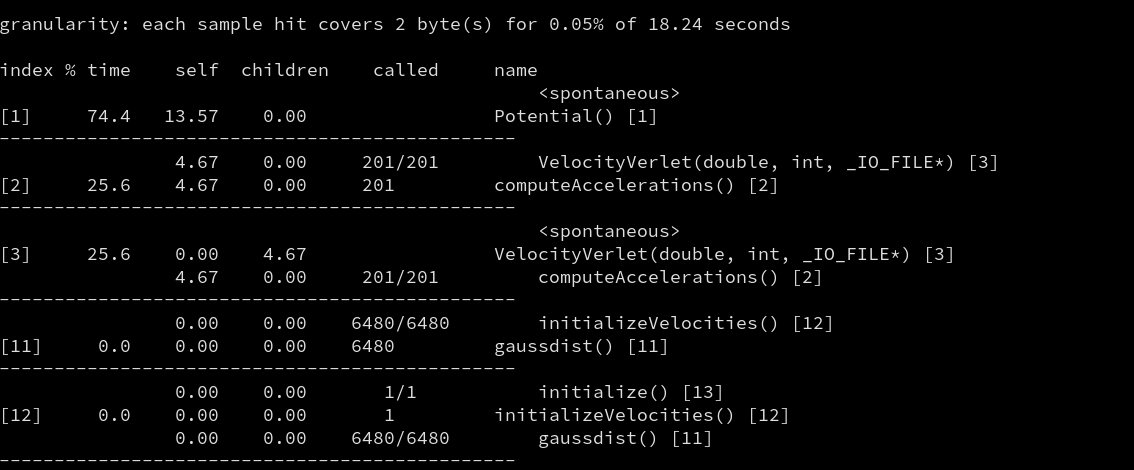
\includegraphics[scale=0.45]{images/gprof_O2_origina_CallGraohl.png}
\caption{Call-graph of the Original Code}
\label{fig}
\end{figure}

\begin{figure}[htbp]
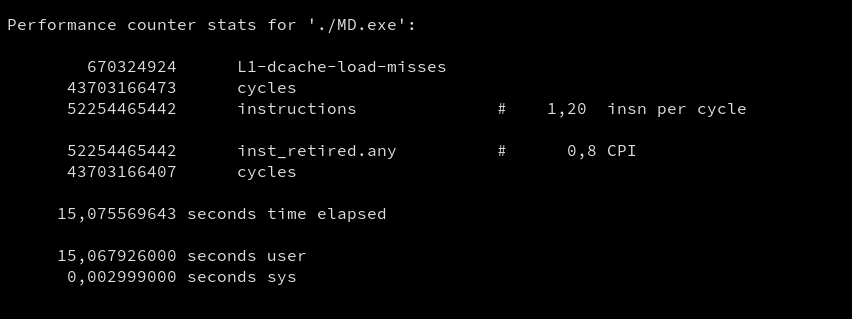
\includegraphics[scale=0.6]{images/Bad_code_no_vect.png}
\caption{Perf Status of the Original Code without vectorization and with the Ofast flag}
\label{fig}
\end{figure}

\begin{figure}[htbp]
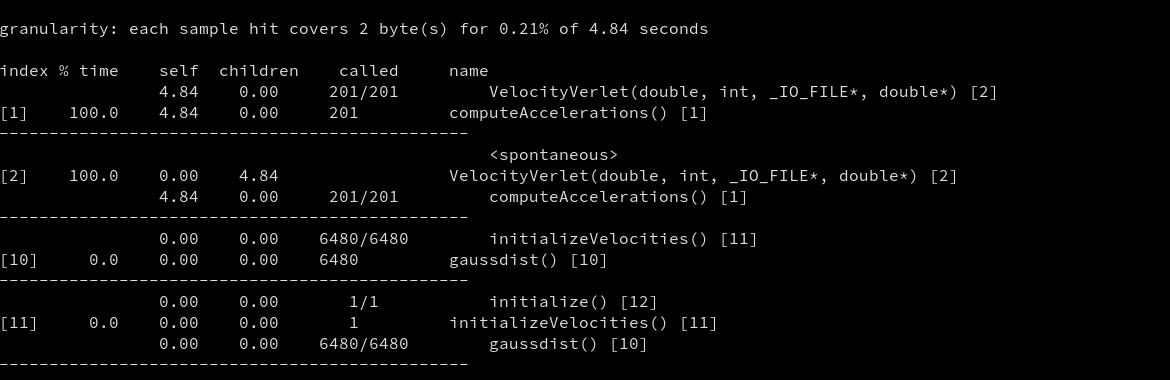
\includegraphics[scale=0.45]{images/Call_graf_latest.png}
\caption{Call-graph of the Optimized Code}
\label{fig}
\end{figure}

\begin{figure}[htbp]
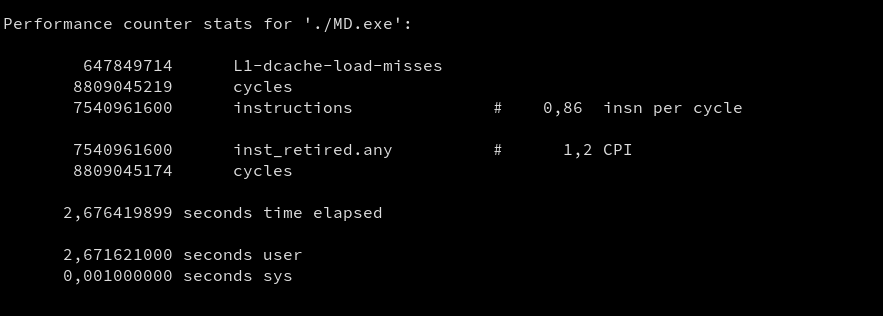
\includegraphics[scale=0.6]{images/2.6.png}
\caption{Perf Status of the Optimized Code with vectorization and the compiler flag Ofast}
\label{fig}
\end{figure}

\begin{figure}[htbp]
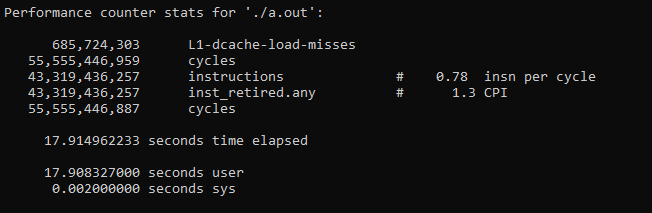
\includegraphics[scale=0.9]{images/ofasstpoooog.png}
\caption{Perf Status of the Original Code with vectorization and the compiler flag Ofast}
\label{fig}
\end{figure}

\begin{figure}[htbp]
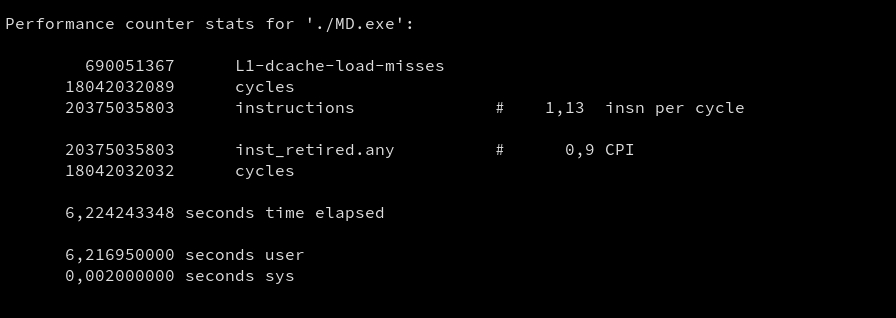
\includegraphics[scale=0.6]{images/Good_code_not_vectorized.png}
\caption{Perf Status of the Optimized Code not vectorized and with Ofast flag}
\label{fig}
\end{figure}

\begin{figure}[htbp]
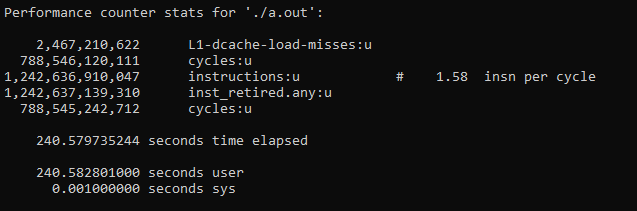
\includegraphics[scale=0.9]{images/deu200.png}
\caption{Perf Status of the Original code with the O2 flag}
\label{fig}
\end{figure}

\begin{figure}[htbp]
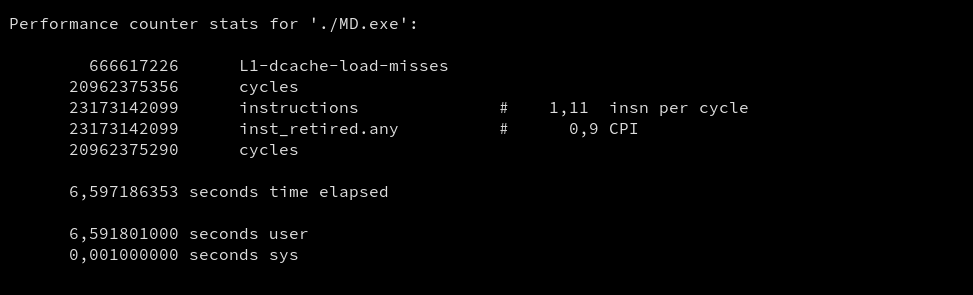
\includegraphics[scale=0.6]{images/Good_code_O2.png}
\caption{Perf Status of the optimized code with the O2 flag}
\label{fig}
\end{figure}

\end{document}
